\documentclass[11pt,a4paper]{report}
\usepackage[textwidth=37em,vmargin=30mm]{geometry}
\usepackage{calc,xunicode,amsmath,amssymb,paralist,enumitem,tabu,booktabs,datetime2,xeCJK,xeCJKfntef,listings}
\usepackage{tocloft,fancyhdr,tcolorbox,xcolor,graphicx,eso-pic,xltxtra,xelatexemoji}

\newcommand{\envyear}[0]{2025}
\newcommand{\envdatestr}[0]{2025-08-21}
\newcommand{\envfinaldir}[0]{webdb/2025/20250821/final}

\usepackage[hidelinks]{hyperref}
\hypersetup{
    colorlinks=false,
    pdfpagemode=FullScreen,
    pdftitle={Web Digest - \envdatestr}
}

\setlength{\cftbeforechapskip}{10pt}
\renewcommand{\cftchapfont}{\rmfamily\bfseries\large\raggedright}
\setlength{\cftbeforesecskip}{2pt}
\renewcommand{\cftsecfont}{\sffamily\small\raggedright}

\setdefaultleftmargin{2em}{2em}{1em}{1em}{1em}{1em}

\usepackage{xeCJK,xeCJKfntef}
\xeCJKsetup{PunctStyle=plain,RubberPunctSkip=false,CJKglue=\strut\hskip 0pt plus 0.1em minus 0.05em,CJKecglue=\strut\hskip 0.22em plus 0.2em}
\XeTeXlinebreaklocale "zh"
\XeTeXlinebreakskip = 0pt


\setmainfont{Brygada 1918}
\setromanfont{Brygada 1918}
\setsansfont{IBM Plex Sans}
\setmonofont{JetBrains Mono NL}
\setCJKmainfont{Noto Serif CJK SC}
\setCJKromanfont{Noto Serif CJK SC}
\setCJKsansfont{Noto Sans CJK SC}
\setCJKmonofont{Noto Sans CJK SC}

\setlength{\parindent}{0pt}
\setlength{\parskip}{8pt}
\linespread{1.15}

\lstset{
	basicstyle=\ttfamily\footnotesize,
	numbersep=5pt,
	backgroundcolor=\color{black!5},
	showspaces=false,
	showstringspaces=false,
	showtabs=false,
	tabsize=2,
	captionpos=b,
	breaklines=true,
	breakatwhitespace=true,
	breakautoindent=true,
	linewidth=\textwidth
}






\newcommand{\coverpic}[2]{
    % argv: itemurl, authorname
    Cover photo by #2~~(\href{#1}{#1})
}
\newcommand{\makeheader}[0]{
    \begin{titlepage}
        % \newgeometry{hmargin=15mm,tmargin=21mm,bmargin=12mm}
        \begin{center}
            
            \rmfamily\scshape
            \fontspec{BaskervilleF}
            \fontspec{Old Standard}
            \fontsize{59pt}{70pt}\selectfont
            WEB\hfill DIGEST
            
            \vfill
            % \vskip 30pt
            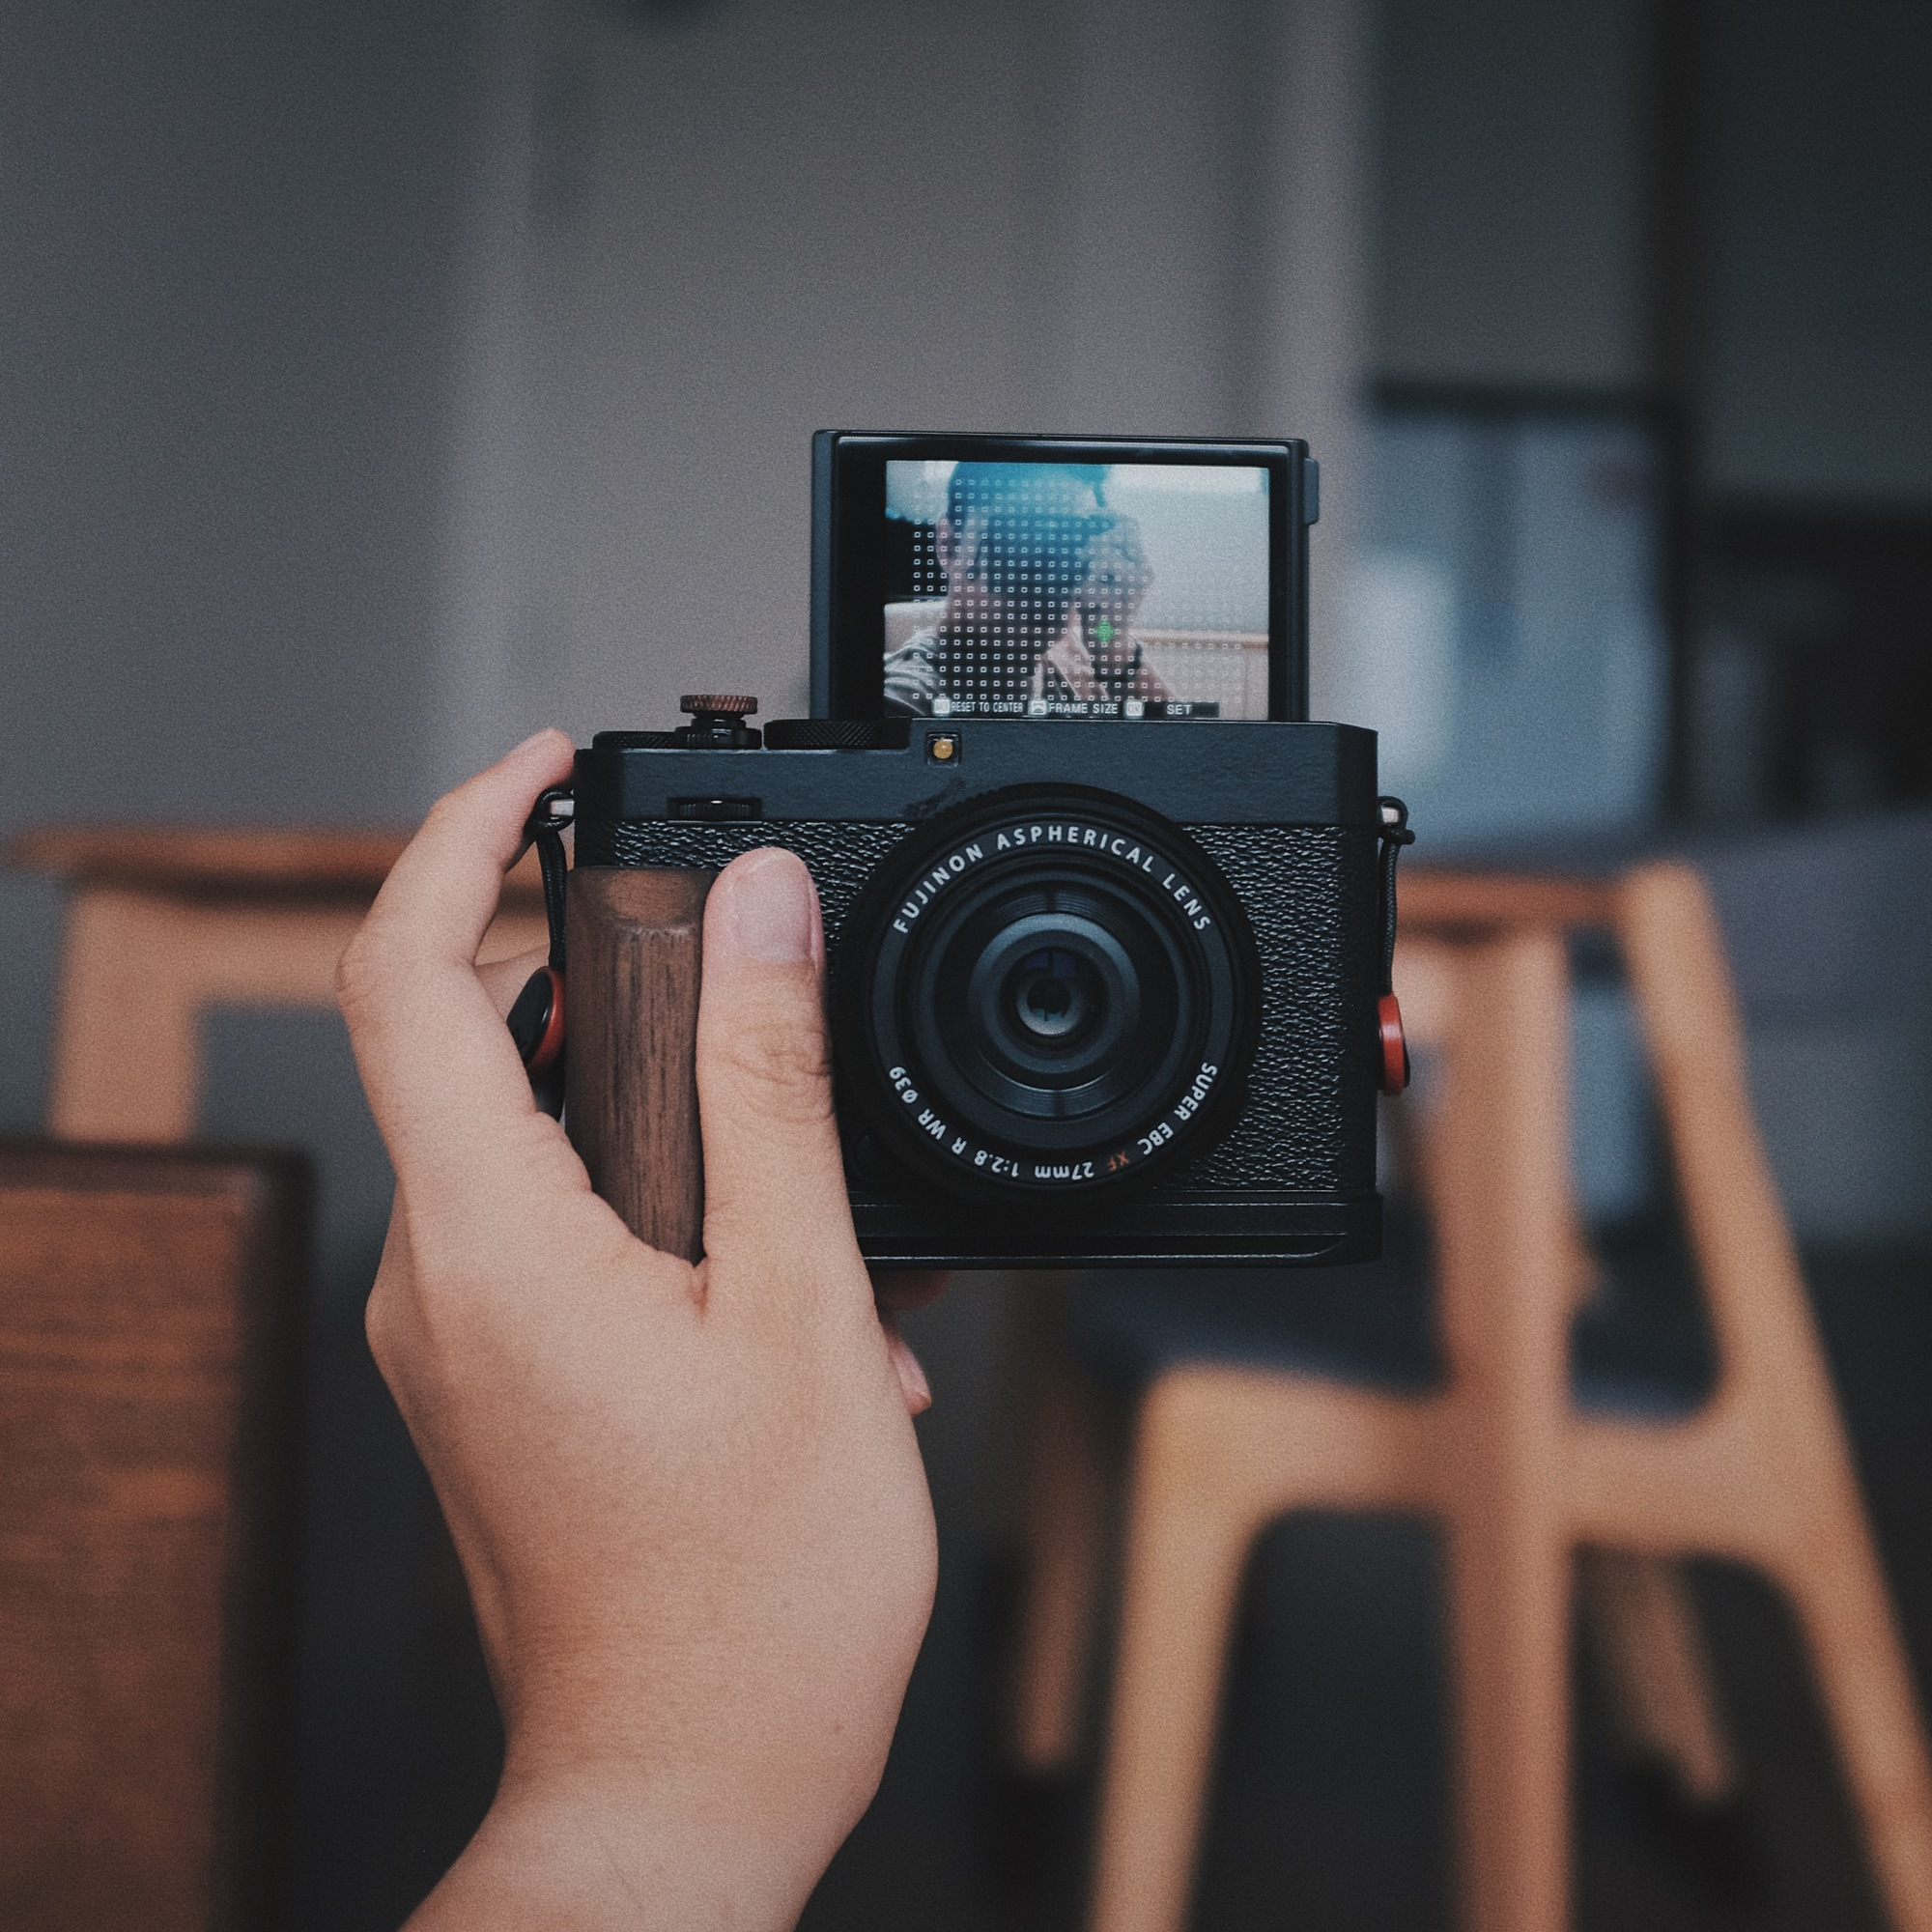
\includegraphics[width=\linewidth]{\envfinaldir/coverpic-prod.jpg}\par
            % \vskip 30pt
            \vfill

            \normalsize\rmfamily\scshape
            \copyright{} The Web Digest Project \hfill\large \envdatestr
        \end{center}
    \end{titlepage}
    % \restoregeometry
}
\newcommand{\simplehref}[1]{%
    \textcolor{blue!80!green}{\href{#1}{#1}}%
}
\renewcommand{\contentsname}{\center\Huge\sffamily\bfseries Contents\par\vskip 20pt}
\newcounter{ipartcounter}
\setcounter{ipartcounter}{0}
\newcommand{\ipart}[1]{
    % \vskip 20pt
    \clearpage
    \stepcounter{ipartcounter}
    \phantomsection
    \addcontentsline{toc}{chapter}{#1}
    % \begin{center}
    %     \Huge
    %     \sffamily\bfseries
    %     #1
    % \end{center}
    % \vskip 20pt plus 7pt
}
\newcounter{ichaptercounter}
\setcounter{ichaptercounter}{0}
\newcommand{\ichapter}[1]{
    % \vskip 20pt
    \clearpage
    \stepcounter{ichaptercounter}
    \phantomsection
    \addcontentsline{toc}{section}{\numberline{\arabic{ichaptercounter}}#1}
    \begin{center}
        \Huge
        \sffamily\bfseries
        #1
    \end{center}
    \vskip 20pt plus 7pt
}
\newcommand{\entrytitlefont}[1]{\subsection*{\raggedright\Large\sffamily\bfseries#1}}
\newcommand{\entryitemGeneric}[2]{
    % argv: title, url
    \parbox{\linewidth}{
        \entrytitlefont{#1}\par\vskip 5pt
        \footnotesize\ttfamily\mdseries
        \simplehref{#2}
    }\vskip 11pt plus 11pt minus 1pt
}
\newcommand{\entryitemGithub}[3]{
    % argv: title, url, desc
    \parbox{\linewidth}{
        \entrytitlefont{#1}\par\vskip 5pt
        \footnotesize\ttfamily\mdseries
        \simplehref{#2}\par\vskip 5pt
        \small\rmfamily\mdseries#3
    }\vskip 11pt plus 11pt minus 1pt
}
\newcommand{\entryitemAp}[3]{
    % argv: title, url, desc
    \parbox{\linewidth}{
        \entrytitlefont{#1}\par\vskip 5pt
        \footnotesize\ttfamily\mdseries
        \simplehref{#2}\par\vskip 5pt
        \small\rmfamily\mdseries#3
    }\vskip 11pt plus 11pt minus 1pt
}
\newcommand{\entryitemHackernews}[3]{
    % argv: title, hnurl, rawurl
    % \parbox{\linewidth}{
    %     \entrytitlefont{#1}\par\vskip 5pt
    %     \footnotesize\ttfamily\mdseries
    %     \simplehref{#3}\par
    %     \textcolor{black!50}{\href{#2}{#2}}
    % }\vskip 11pt plus 11pt minus 1pt
    \begin{minipage}{\linewidth}
            \entrytitlefont{#1}\par\vskip 5pt
            \footnotesize\ttfamily\mdseries
            \simplehref{#3}\par
            \textcolor{black!50}{\href{#2}{#2}}
    \end{minipage}\par\vskip 11pt plus 11pt minus 1pt
}







\begin{document}

\makeheader

\tableofcontents\clearpage




\ipart{Developers}
\ichapter{Hacker News}
\entryitemTwoLinks{Introduction to AT Protocol}{https://news.ycombinator.com/item?id=44965233}{https://mackuba.eu/2025/08/20/introduction-to-atproto/}

\entryitemTwoLinks{Zedless: Zed fork focused on privacy and being local-first}{https://news.ycombinator.com/item?id=44964916}{https://github.com/zedless-editor/zed}

\entryitemTwoLinks{Pixel 10 Phones}{https://news.ycombinator.com/item?id=44963939}{https://blog.google/products/pixel/google-pixel-10-pro-xl/}

\entryitemTwoLinks{An Update on Pytype}{https://news.ycombinator.com/item?id=44963724}{https://github.com/google/pytype}

\entryitemTwoLinks{Digg.com is back}{https://news.ycombinator.com/item?id=44963430}{https://www.digg.com/}

\entryitemTwoLinks{OPA maintainers and Styra employees hired by Apple}{https://news.ycombinator.com/item?id=44962969}{https://blog.openpolicyagent.org/note-from-teemu-tim-and-torin-to-the-open-policy-agent-community-2dbbfe494371}

\entryitemTwoLinks{Closer to the Metal: Leaving Playwright for CDP}{https://news.ycombinator.com/item?id=44962869}{https://browser-use.com/posts/playwright-to-cdp}

\entryitemTwoLinks{AWS in 2025: Stuff you think you know that's now wrong}{https://news.ycombinator.com/item?id=44962844}{https://www.lastweekinaws.com/blog/aws-in-2025-the-stuff-you-think-you-know-thats-now-wrong/}

\entryitemTwoLinks{Why are anime catgirls blocking my access to the Linux kernel?}{https://news.ycombinator.com/item?id=44962529}{https://lock.cmpxchg8b.com/anubis.html}

\entryitemTwoLinks{Show HN: I was curious about spherical helix, ended up making this visualization}{https://news.ycombinator.com/item?id=44962066}{https://visualrambling.space/moving-objects-in-3d/}

\entryitemTwoLinks{Gemma 3 270M re-implemented in pure PyTorch for local tinkering}{https://news.ycombinator.com/item?id=44962059}{https://github.com/rasbt/LLMs-from-scratch/tree/main/ch05/12\_gemma3}

\entryitemTwoLinks{Sequoia backs Zed}{https://news.ycombinator.com/item?id=44961172}{https://zed.dev/blog/sequoia-backs-zed}

\entryitemTwoLinks{Show HN: Project management system for Claude Code}{https://news.ycombinator.com/item?id=44960594}{https://github.com/automazeio/ccpm}

\entryitemTwoLinks{Tidewave Web: in-browser coding agent for Rails and Phoenix}{https://news.ycombinator.com/item?id=44960316}{https://tidewave.ai/blog/tidewave-web-phoenix-rails}

\entryitemTwoLinks{Mirrorshades: The Cyberpunk Anthology (1986)}{https://news.ycombinator.com/item?id=44959833}{https://www.rudyrucker.com/mirrorshades/HTML/}

\entryitemTwoLinks{Databricks is raising a Series K Investment at >\$100B valuation}{https://news.ycombinator.com/item?id=44959092}{https://www.databricks.com/company/newsroom/press-releases/databricks-raising-series-k-investment-100-billion-valuation}

\entryitemTwoLinks{Ask HN: Why does the US Visa application website do a port-scan of my network?}{https://news.ycombinator.com/item?id=44959073}{https://news.ycombinator.com/item?id=44959073}

\entryitemTwoLinks{Analysis of the GFW's Unconditional Port 443 Block on August 20, 2025}{https://news.ycombinator.com/item?id=44958621}{https://gfw.report/blog/gfw\_unconditional\_rst\_20250820/en/}

\entryitemTwoLinks{Modern CI is too complex and misdirected (2021)}{https://news.ycombinator.com/item?id=44958400}{https://gregoryszorc.com/blog/2021/04/07/modern-ci-is-too-complex-and-misdirected/}

\entryitemTwoLinks{We're Not So Special: A new book challenges human exceptionalism}{https://news.ycombinator.com/item?id=44958145}{https://democracyjournal.org/magazine/78/were-not-so-special/}\ichapter{Phoronix}
\entryitemGeneric{\hskip 0pt{}Libre-Chip Awarded NLnet Grant To Prototype A CPU That Isn't Vulnerable To Spectre Flaws}{https://www.phoronix.com/news/Libre-Chip-NLnet-Grant}

\entryitemGeneric{\hskip 0pt{}systemd 259 To Raise Linux System Requirements}{https://www.phoronix.com/news/systemd-259-Requirements}

\entryitemGeneric{\hskip 0pt{}AMD FidelityFX SDK 2.0 Released With FSR 4 Included}{https://www.phoronix.com/news/AMD-FidelityFX-SDK-2.0}

\entryitemGeneric{\hskip 0pt{}Mesa 25.2.1 Released: Restores NVK On Kepler, Additional Intel Battlemage ID}{https://www.phoronix.com/news/Mesa-25.2.1-Released}

\entryitemGeneric{\hskip 0pt{}MoltenVK 1.4 Released For Bringing Vulkan 1.4 To macOS Atop Metal}{https://www.phoronix.com/news/MoltenVK-1.4}

\entryitemGeneric{\hskip 0pt{}Ubuntu 25.10 ARM64 Desktop ISO Aims For Better Hardware Experience With "Stubble"}{https://www.phoronix.com/news/Ubuntu-25.10-ARM64-Stubble}

\entryitemGeneric{\hskip 0pt{}LibreOffice 25.8 Released With UI Enhancements, Better Performance}{https://www.phoronix.com/news/LibreOffice-25.8-Released}

\entryitemGeneric{\hskip 0pt{}AMD EPYC 9005 Squeezes Out More Performance On Linux 6.17}{https://www.phoronix.com/news/AMD-EPYC-9005-Linux-6.17}

\entryitemGeneric{\hskip 0pt{}Linux 6.18 To Introduce New Driver For TASCAM US-144MKII USB Audio Interface}{https://www.phoronix.com/news/Linux-Driver-TASCAM-US-144MKII}


\ipart{Developers~~~~(zh-Hans)}
\ichapter{Solidot}
\entryitemGeneric{\hskip 0pt{}AWS CEO 称用 AI 取代初级员工是蠢主意}{https://www.solidot.org/story?sid=82100}

\entryitemGeneric{\hskip 0pt{}Firefox 142.0 释出}{https://www.solidot.org/story?sid=82099}

\entryitemGeneric{\hskip 0pt{}苹果将在印度组装更多新款 iPhone }{https://www.solidot.org/story?sid=82098}

\entryitemGeneric{\hskip 0pt{}印度有时间先富后老}{https://www.solidot.org/story?sid=82097}

\entryitemGeneric{\hskip 0pt{}北极一群岛的冰融化量足以使海平面上升 0.16 毫米}{https://www.solidot.org/story?sid=82096}

\entryitemGeneric{\hskip 0pt{}电流重塑角膜能有效矫正视力}{https://www.solidot.org/story?sid=82095}

\entryitemGeneric{\hskip 0pt{}Copilot 对文件的访问会不记录在日志内}{https://www.solidot.org/story?sid=82094}

\entryitemGeneric{\hskip 0pt{}巴基斯坦互联网连接速度降至平常的五分之一}{https://www.solidot.org/story?sid=82093}

\entryitemGeneric{\hskip 0pt{}中国 HTTPS 访问短暂受限}{https://www.solidot.org/story?sid=82092}

\entryitemGeneric{\hskip 0pt{}为什么好莱坞停止制作喜剧片}{https://www.solidot.org/story?sid=82091}

\entryitemGeneric{\hskip 0pt{}部分 Docker 镜像仍然包含 XZ Utils 后门 }{https://www.solidot.org/story?sid=82090}

\entryitemGeneric{\hskip 0pt{}软银向英特尔投资 20 亿美元}{https://www.solidot.org/story?sid=82089}

\entryitemGeneric{\hskip 0pt{}MIT 报告称 95\% 的企业生成式 AI 试验失败了}{https://www.solidot.org/story?sid=82088}

\entryitemGeneric{\hskip 0pt{}中国有望在美国之前登陆月球}{https://www.solidot.org/story?sid=82087}

\entryitemGeneric{\hskip 0pt{}英国官员想要阻止儿童使用 VPN 浏览成人内容}{https://www.solidot.org/story?sid=82086}

\entryitemGeneric{\hskip 0pt{}证据显示地球之水起源于彗星}{https://www.solidot.org/story?sid=82085}

\entryitemGeneric{\hskip 0pt{}医生救回几乎``身首离断''患者}{https://www.solidot.org/story?sid=82084}

\entryitemGeneric{\hskip 0pt{}基因改变果蝇的求爱方式}{https://www.solidot.org/story?sid=82083}

\entryitemGeneric{\hskip 0pt{}卫星捕捉到 8.8 级地震所引发海啸的细节}{https://www.solidot.org/story?sid=82082}

\entryitemGeneric{\hskip 0pt{}83\% 的 Python 开发者仍然使用旧版本}{https://www.solidot.org/story?sid=82081}\ichapter{V2EX}
\entryitemGeneric{\hskip 0pt{}[macOS] 如何清理 word 生成的``~\$''前缀的隐藏文件}{https://www.v2ex.com/t/1153833}

\entryitemGeneric{\hskip 0pt{}[信息安全] PVE 防火墙开启 IP Filter + MAC Filter 能有效防御 ARP 攻击吗?在 PVE 论坛找到的帖子说可以,但是 GPT 告诉我不可以,因为 ARP 攻击发生在第 2 层而软件防火墙工作在第三层}{https://www.v2ex.com/t/1153832}

\entryitemGeneric{\hskip 0pt{}[分享发现] 一个 trx 能量机器人,节约很多手续费。}{https://www.v2ex.com/t/1153831}

\entryitemGeneric{\hskip 0pt{}[酷工作] AI 创业公司 iOS 招聘 [深圳/熟悉后可远程]}{https://www.v2ex.com/t/1153830}

\entryitemGeneric{\hskip 0pt{}[浏览器] 老外有人开发象 Via 这样的迷你安卓浏览器吗?}{https://www.v2ex.com/t/1153829}

\entryitemGeneric{\hskip 0pt{}[酷工作] [远程 ]Flutter 开发工程师, 远程全职 2 名, 预算 ¥10k-20k/m}{https://www.v2ex.com/t/1153828}

\entryitemGeneric{\hskip 0pt{}[OpenAI] chatgpt 的 app 是不是挂了?}{https://www.v2ex.com/t/1153827}

\entryitemGeneric{\hskip 0pt{}[宽带症候群] 近期高墙事件}{https://www.v2ex.com/t/1153826}

\entryitemGeneric{\hskip 0pt{}[Android] 安卓有没有过代理检测的插件}{https://www.v2ex.com/t/1153825}

\entryitemGeneric{\hskip 0pt{}[生活] 邻居家的狗影响到我该怎么办?}{https://www.v2ex.com/t/1153823}

\entryitemGeneric{\hskip 0pt{}[天黑以后] 20250825 午夜俱乐部}{https://www.v2ex.com/t/1153822}

\entryitemGeneric{\hskip 0pt{}[问与答] 关于暴龙镜框}{https://www.v2ex.com/t/1153821}

\entryitemGeneric{\hskip 0pt{}[Visual Studio Code] VSCode 有没有稳定好用的 AI 插件}{https://www.v2ex.com/t/1153820}

\entryitemGeneric{\hskip 0pt{}[程序员] 我覺得 Ruby 最優秀的地方(RSpec)}{https://www.v2ex.com/t/1153819}

\entryitemGeneric{\hskip 0pt{}[问与答] 晚上喝多了,把小姨子认成老婆了……唉}{https://www.v2ex.com/t/1153818}

\entryitemGeneric{\hskip 0pt{}[OpenAI] 现阶段 AI,有没有生成视频质量比较好的开源大模型}{https://www.v2ex.com/t/1153817}

\entryitemGeneric{\hskip 0pt{}[分享发现] 7 个超实用 AI 写论文工具测评推荐}{https://www.v2ex.com/t/1153816}

\entryitemGeneric{\hskip 0pt{}[问与答] 准备美签二签,求分享下经验}{https://www.v2ex.com/t/1153815}

\entryitemGeneric{\hskip 0pt{}[问与答] 想咨询下各位 v 友这家公司不知道要不要去?}{https://www.v2ex.com/t/1153814}

\entryitemGeneric{\hskip 0pt{}[OpenAI] 在线体验 GPT-OSS、GPT-5 的两个对话网址(OpenAI 官方 VS 山寨)}{https://www.v2ex.com/t/1153812}

\entryitemGeneric{\hskip 0pt{}[分享发现] 除了打游戏,刷短视频,聚众喝酒,独居码农有无乐子可搞}{https://www.v2ex.com/t/1153811}

\entryitemGeneric{\hskip 0pt{}[职场话题] 一起来分析下这家公司 HR 的真实想法}{https://www.v2ex.com/t/1153810}

\entryitemGeneric{\hskip 0pt{}[分享发现] 写论文不用愁!这 6 个 AI 论文写作工具推荐给你}{https://www.v2ex.com/t/1153808}

\entryitemGeneric{\hskip 0pt{}[Solana] Ledger 回复我说是 V 站没集成人家,哈哈哈}{https://www.v2ex.com/t/1153807}

\entryitemGeneric{\hskip 0pt{}[远程工作] 为了方便 交流远程工作}{https://www.v2ex.com/t/1153806}

\entryitemGeneric{\hskip 0pt{}[分享创造] 做了一个图片编辑的网站,支持用自然语言修改图片}{https://www.v2ex.com/t/1153805}

\entryitemGeneric{\hskip 0pt{}[问与答] 理性讨论中文语境下哪种数字表现形式易读?}{https://www.v2ex.com/t/1153804}

\entryitemGeneric{\hskip 0pt{}[问与答] 大家看短剧么?都去哪里看?}{https://www.v2ex.com/t/1153802}

\entryitemGeneric{\hskip 0pt{}[生活] 你好陌生人,可以祝我生日快乐吗}{https://www.v2ex.com/t/1153801}

\entryitemGeneric{\hskip 0pt{}[分享发现] 沉浸式翻译, Grok 来找你了,泄露超 37 万用户聊天记录}{https://www.v2ex.com/t/1153800}

\entryitemGeneric{\hskip 0pt{}[全球工单系统] 鸿蒙手机系统有 SIM 缺陷问题}{https://www.v2ex.com/t/1153799}

\entryitemGeneric{\hskip 0pt{}[分享创造] 卧槽,再也不用来回上传和裁剪微信公众号文章封面了}{https://www.v2ex.com/t/1153796}

\entryitemGeneric{\hskip 0pt{}[宠物] 有人要买猫吗}{https://www.v2ex.com/t/1153795}

\entryitemGeneric{\hskip 0pt{}[问与答] 火狐标签页还能恢复吗}{https://www.v2ex.com/t/1153794}

\entryitemGeneric{\hskip 0pt{}[Solana] 设置里,连接 solana 钱包应该接一个 wallet connect}{https://www.v2ex.com/t/1153793}

\entryitemGeneric{\hskip 0pt{}[跑步] 有没有人玩过通过两个手指的节奏来控制跑步的小游戏吗}{https://www.v2ex.com/t/1153792}

\entryitemGeneric{\hskip 0pt{}[问与答] 软件工程专业毕设,写微信小程序好吗?}{https://www.v2ex.com/t/1153791}

\entryitemGeneric{\hskip 0pt{}[摄影] 之前随手拍的招聘,才发现做壁纸很合适}{https://www.v2ex.com/t/1153790}

\entryitemGeneric{\hskip 0pt{}[生活] 便宜的像不要钱一样的电信套餐}{https://www.v2ex.com/t/1153789}

\entryitemGeneric{\hskip 0pt{}[问与答] 有不有大佬知道怎么 接单,最近日子过的太顺了想给自己添堵(}{https://www.v2ex.com/t/1153788}

\entryitemGeneric{\hskip 0pt{}[问与答] 你身上没有设备供你传输翻墙工具给别人,你该如何帮助身边的人顺利翻墙}{https://www.v2ex.com/t/1153787}

\entryitemGeneric{\hskip 0pt{}[Apple] Chuckle 第三方 X 客户端 原微博客户端 Share 开发者}{https://www.v2ex.com/t/1153785}

\entryitemGeneric{\hskip 0pt{}[Claude] claude code 自定义 api 遇到问题}{https://www.v2ex.com/t/1153784}

\entryitemGeneric{\hskip 0pt{}[问与答] 作为一个传统的软件开发者,现在入局学习 cnn 等深度网络迟吗}{https://www.v2ex.com/t/1153783}

\entryitemGeneric{\hskip 0pt{}[分享发现] 我的香港银行账户与美国银行账户之路,经验与教训}{https://www.v2ex.com/t/1153782}

\entryitemGeneric{\hskip 0pt{}[前端开发] 有大佬们遇到过移动端缩放问题么}{https://www.v2ex.com/t/1153781}

\entryitemGeneric{\hskip 0pt{}[分享发现] AI 生成 Labubu 风格图片}{https://www.v2ex.com/t/1153780}

\entryitemGeneric{\hskip 0pt{}[职场话题] 技术会议安利 \& 演讲征集: 2025 杭州 Kubernetes Community Days}{https://www.v2ex.com/t/1153779}

\entryitemGeneric{\hskip 0pt{}[程序员] apple 开发的对账单没有税跟苹果费数据吗?}{https://www.v2ex.com/t/1153778}

\entryitemGeneric{\hskip 0pt{}[汽车] v 友们,这种情况,是不是应该放弃油车,买电车?}{https://www.v2ex.com/t/1153777}


\ipart{Generic News}







\clearpage
\leavevmode\vfill
\footnotesize

Copyright \copyright{} 2023-2025 Neruthes and other contributors.

This document is published with CC BY-NC-ND 4.0 license.

The entries listed in this newsletter may be copyrighted by their respective creators.

This newsletter is generated by the Web Digest project.

The newsletters are also delivered via Telegram channel \CJKunderline{\href{https://t.me/webdigestchannel}{https://t.me/webdigestchannel}}.\\
RSS feed is available at \CJKunderline{\href{https://webdigest.pages.dev/rss.xml}{https://webdigest.pages.dev/rss.xml}}.

This newsletter is available in PDF at
\CJKunderline{\href{https://webdigest.pages.dev/}{https://webdigest.pages.dev/}}.

The source code being used to generate this newsletter is available at\\
\CJKunderline{\href{https://github.com/neruthes/webdigest}{https://github.com/neruthes/webdigest}}.

This newsletter is also available in
\CJKunderline{\href{http://webdigest.pages.dev/readhtml/\envyear/WebDigest-20250821.html}{HTML}} and
\CJKunderline{\href{https://github.com/neruthes/webdigest/blob/master/markdown/\envyear/WebDigest-20250821.md}{Markdown}}.


\coverpic{https://unsplash.com/photos/the-sun-sets-over-the-ocean-a-beautiful-sight-vBi5MfgGg64}{Barbare Kacharava}


\end{document}
